\section{Giao diện người dùng}
Giao diện người dùng của ứng dụng webfuzzer được xây dựng dựa trên bản mẫu (template) React Reduction \parencite{react-reduction-github}. Bản mẫu này được viết trên React.js với sự hỗ trợ của thư viện reactstrap\footnote{\href{https://reactstrap.github.io/}{Nguồn: https://reactstrap.github.io/}}, hiện thực sẵn một số thành phần như thanh điều hướng, các nút bấm, ô lựa chọn, bảng biểu, kiểu chữ,... cũng như giao diện mặc định đẹp mắt, dễ dàng chỉnh sửa theo nhu cầu lập trình. Công việc của chúng tôi là hiện thực và thiết lập luồng hoạt động của ba thành phần chính của \acrshort{ui}, đảm nhiệm được việc gọi các \acrshort{api} backend cung cấp và xử lí kết quả trả về, hiển thị được những thông tin cần thiết đồng thời đáp ứng nhu cầu kiểm thử của người dùng như yêu cầu và thiết kế \acrshort{ui} đã đề ra ở \textbf{Chương 5}.\par
React.js là một khung thức lập trình giao diện người dùng hướng thành phần (component-based), mỗi trang web và các thành phần nhỏ hơn trong trang đa phần đều kế thừa các class có sẵn của React.js và được hiện thực dưới dạng các component. Mỗi component có tập các trạng thái riêng (state) và tập những thuộc tính được truyền vào (props). Bản thân một component trong React.js sẽ chỉ thay đổi được state của nó bằng phương thức \texttt{setState} chứ không thay đổi được giá trị của những props mà nó được nhận. Mỗi khi hàm \texttt{setState} thực hiện xong, phương thức \texttt{render} của component đó sẽ được khởi chạy, tải lại nội dung hiển thị của component theo những giá trị state mới mà không làm mới lại cả trang web. Phương thức \texttt{render} của các component trả về giá trị là các JSX, gồm những đoạn mã \acrshort{html} hoặc các component lồng với JavaScript đặc trưng của khung thức này, tương ứng với nội dung hiển thị của component đó ở giao diện người dùng.\par
Trước tiên, trong quá trình hiện thực \acrshort{ui} của ứng dụng, chúng tôi sử dụng thư viện Axios\footnote{\href{https://www.npmjs.com/package/axios}{Nguồn: https://www.npmjs.com/package/axios}} để tương tác với các \acrshort{api} ở backend ứng dụng webfuzzer. Thư viện này hỗ trợ gửi và nhận các thông điệp \acrshort{http} một cách đơn giản thông qua việc cung cấp các tham số cần thiết như đường dẫn \acrshort{api}, phương thức \acrshort{http} kèm theo body và các tham số nếu có. Những lời gọi \acrshort{api} này nằm trong các đoạn mã xử lí sự kiện của JSX khi người dùng tương tác với giao diện và khi tải nội dung trang. Đoạn mã \ref{lst:call-API-from-UI} sau hiện thực việc gọi API và lấy ra kết quả trả về trong mã nguồn \acrshort{ui}.
\begin{lstlisting}[style=ES6, label={lst:call-API-from-UI}, caption={Gọi API từ mã nguồn UI}]
import axios from 'axios';
const BASE_URL = require('./globalConfig').BASE_URL;
const callApi = async (endpoint, method = 'get', body) => {
  try {
      let { data } = await axios({
        method: method,
        url: `${BASE_URL}${endpoint}`,
        data: body
      });
      return data;
  } catch (err) {
      console.log(err);
      return null;
  }
}
\end{lstlisting}
Để điều hướng hai trang web chính của \acrshort{ui}, chúng tôi sử dụng các component \texttt{Switch, Route} có sẵn của React.js trong Đoạn mã \ref{lst:routing-at-ui} sau.
\begin{lstlisting}[style=ES6, label={lst:routing-at-ui}, caption={Điều hướng các trang web trên \acrshort{ui} của webfuzzer}]
<Switch>
  <MainLayout breakpoint={this.props.breakpoint}>
    <React.Suspense fallback={<PageSpinner />}>
      <Route exact path="/" component={DashboardPage} />
      <Route exact path="/result" component={ResultPage} />
    </React.Suspense>
  </MainLayout>
  <Redirect to="/" />
</Switch>
\end{lstlisting}
Giả sử \acrshort{ui} của ứng dụng webfuzzer được triển khai ở cổng 3000 của máy chủ có địa chỉ IP \texttt{61.28.235.183}. Khi đó, địa chỉ web \texttt{http://61.28.235.183:3000/} sẽ dẫn đến component trang bảng điều khiển và đường dẫn \texttt{http://61.28.235.183:3000/result} dẫn đến component trang kết quả kiểm thử của ứng dụng.
\subsection{Trang bảng điều khiển}
Đầu tiên khi tải trang bảng điều khiển xuống, người dùng cần có sẵn danh sách các request mẫu và loại lỗ hổng cần kiểm thử để chọn tạo yêu cầu kiểm thử. Để làm được điều này, ta gọi các \acrshort{api} \colorbox{gray!30}{\texttt{GET /}} và \colorbox{gray!30}{\texttt{GET /target/configs}} trong phương thức \texttt{componentDidMount} của component, phương thức này luôn chạy đầu tiên mỗi khi component chứa nó được gọi đến. Đoạn mã \ref{lst:component-did-mount} sau là phương thức \texttt{componentDidMount} của component trang bảng điều khiển, lấy các danh sách cần thiết từ \acrshort{api} và lưu vào state của component này.
\begin{lstlisting}[style=ES6, label={lst:component-did-mount}, caption={Hiện thực các thành phần của trang bảng điều khiển}]
componentDidMount = async () => {
	let apiList = [this.getListEndpoints(), this.getVulneTypes()]
	let [res1, res2] = await Promise.all(apiList);
}
getListEndpoints = async (limit = 5, offset = 0) => {
  ...
  let endpointList = await callApi(endpoints.getAllEndpoinst(limit, offset), 'get', null);
  if (endpointList && endpointList.results) {
    let list = endpointList.results.endpointList;
    this.setState({
      endpointsList: list,
      totalRecord: endpointList.results.total
    });
  }
  ...
}
getVulneTypes = async () => {
  ...
  let { results } = await callApi(endpoints.getListVulnes, 'get', null);
  let arr = [];
  if (results) {
    Object.keys(results).forEach((key, idx) => {
      let vulne = {
        id: String(key),
        label: results[key].label,
        check: false,
        type: key === '6' ? 'common' : 'auto'
      }
      arr.push(vulne);
    })
  }
  this.setState({ vulneTypes: [...arr] });
  ...
}
\end{lstlisting}
Theo thiết kế giao diện đã đề ra ở \textbf{Chương 5}, trang này cần ba khung để hiển thị danh sách request mẫu, chi tiết request mẫu, khung chọn lỗ hổng cần kiểm thử và một nút nhấn để tạo yêu cầu kiểm thử. Phương thức \texttt{render} của component này căn chỉnh các khung vuông vức bằng các thành phần (component) \texttt{Row, Column} trong Layout của thư viện reactstrap cùng với \acrshort{css} như Đoạn mã \ref{lst:implement-dashboard-page} sau.
\begin{lstlisting}[style=ES6, label={lst:implement-dashboard-page}, caption={Phương thức \texttt{render} của trang bảng điều khiển}]
<Page
  className="DashboardPage"
  title="Dashboard"
>
  <Row>
    <Col lg="4">
      <EndpointsComponent
        endpointsList={this.state.endpointsList}
        selectEndpoint={this.selectEndpoint}
        endpointSelected={this.state.endpointSelected}
        getListEndpoints={this.getListEndpoints}
        loading={this.state.loading}
        totalRecord={this.state.totalRecord}
      />
    </Col>
    <Col lg="8">
      <BaseRequestComponent selectedEndpoint={this.state.endpointSelected} />
    </Col>
  </Row>
  <Row>
    <Col lg="4">
      <ListVulnes
        listVulnes={this.state.vulneTypes}
        selectVulne={this.selectVulne}
        checkedAllAutoFuzz={this.state.checkedAllAutoFuzz}
        toogleAllAutoFuzz={this.toogleAllAutoFuzz}
      />
      <div className="btn-submit">
        {this.state.loadingSubmit ?
          <AwaitingComponent /> :
          <button
            disabled={!this.state.endpointSelected.Id}
            onClick={() => this.submitFuzzRequest()}>Create fuzz request
        </button>}
      </div>
    </Col>
    <Col lg="8"></Col>
  </Row>
</Page>
\end{lstlisting}
Khung chứa danh sách request mẫu tương ứng với component \texttt{EndpointsComponent} và khung hiển thị nội dung request mẫu tương đương ứng component \texttt{BaseRequestComponent}. Component \texttt{EndpointsComponent} sẽ lưu lại ID của request mẫu đang được chọn vào state \texttt{endpointSelected}, đồng thời component \texttt{BaseRequestComponent} sẽ hiển thị nội dung của request mẫu có ID đó ở bên cạnh. Danh sách các request mẫu sẽ được phân thành nhiều trang để đảm bảo bố cục trang web, mỗi trang gồm 5 request mẫu, việc hiện thực cơ chế phân trang này sẽ được để cập ở \textbf{Đề mục 6.2.3}. Mỗi khung trên được đặt trong một component \texttt{Col} riêng và cả hai nằm trong cùng một component \texttt{Row} trong mã nguồn để nằm ngang hàng nhau trên \acrshort{ui} như Hình \ref{fig:dashboard-ui} sau.
\FloatBarrier
\begin{sidewaysfigure}[!htb]
    \centering
        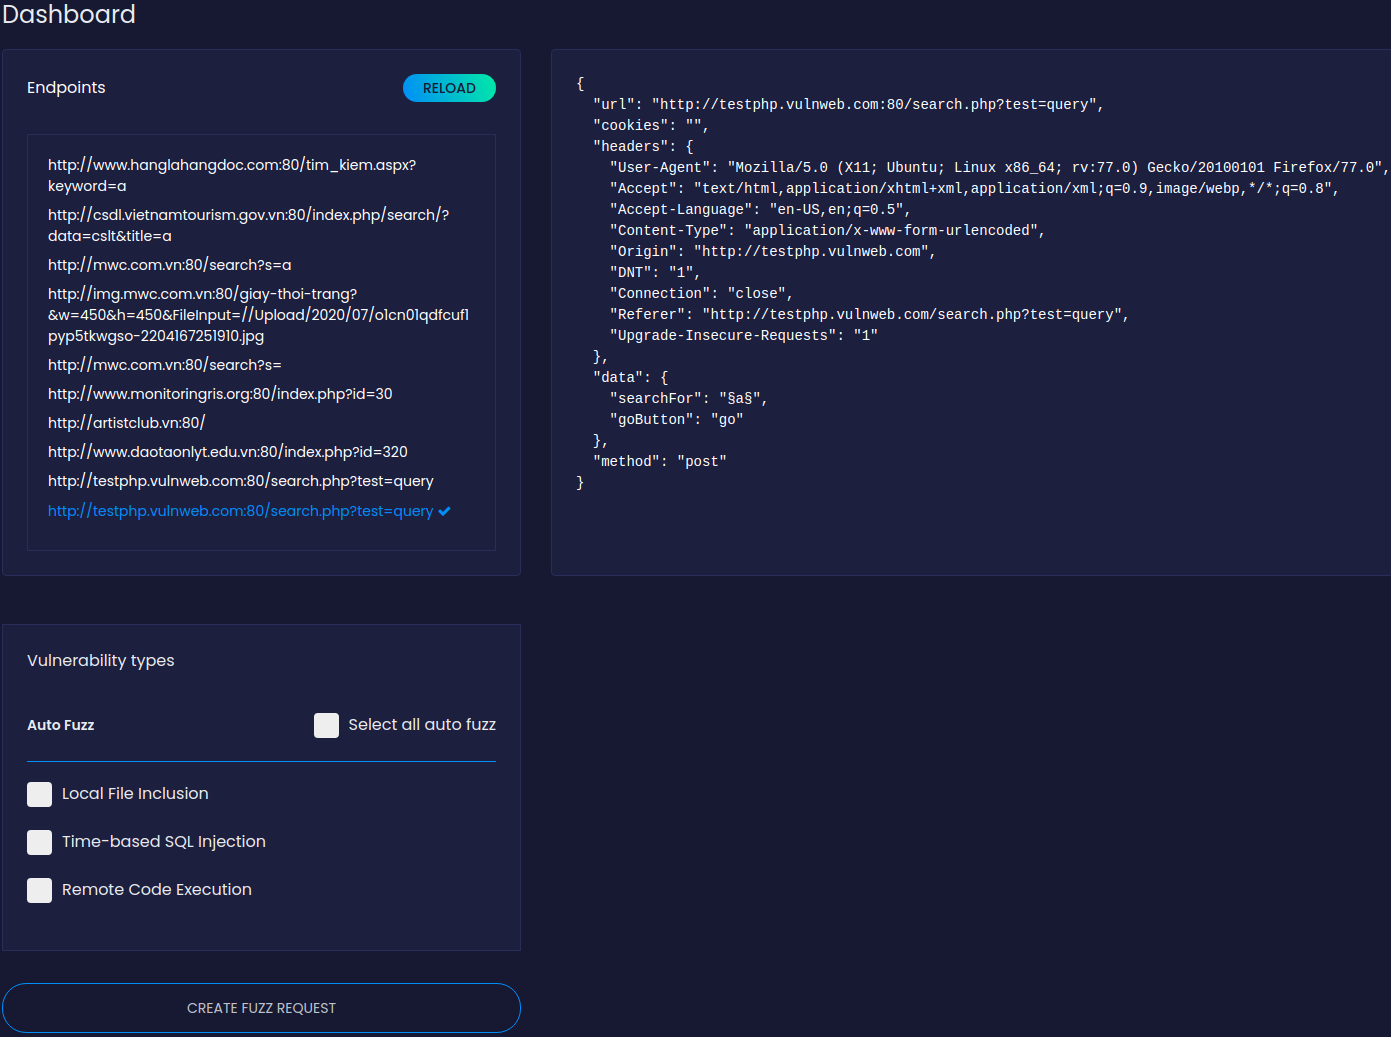
\includegraphics[scale=0.45,keepaspectratio=true]{images/dashboard-ui.png}
    \caption{Giao diện trang bảng điều khiển ở UI ứng dụng webfuzzer}
    \label{fig:dashboard-ui}
\end{sidewaysfigure}
\FloatBarrier
Tương tự, khung chọn loại lỗ hổng kiểm thử tương ứng với component \texttt{ListVulnes} và nút tạo yêu cầu kiểm thử ứng với thẻ \texttt{<div className="btn-submit">} trong mã nguồn. Các thuộc tính \texttt{lg="4"} và \texttt{lg="8"} của component \texttt{Col} mô tả chiều rộng của các khung trên \acrshort{ui}. Hàm xử lí sự kiện \texttt{onClick} nhấn nút này là hàm \texttt{this.submitFuzzRequest()}, có chức năng gọi đến \acrshort{api} \colorbox{gray!30}{\texttt{POST /target}} để tạo yêu cầu kiểm thử dựa trên request mẫu và những loại lỗ hổng đã chọn.
\subsection{Trang kết quả kiểm thử}
Tương tự như trang bảng điều khiển, phương thức \texttt{componentDidMount} của trang sẽ gọi \acrshort{api}\\\colorbox{gray!30}{\texttt{GET /target/list}} để lấy danh sách các yêu cầu kiểm thử cần hiển thị. Bố cục chính của trang là một bảng gồm nhiều hàng, mỗi hàng bao gồm thông tin cơ bản của một yêu cầu kiểm thử và một nút xổ xuống thông tin chi tiết của yêu cầu đó, và một khung tìm kiếm yêu cầu kiểm thử theo \acrshort{url} của request mẫu. Chúng tôi sử dụng thẻ \texttt{table} cùng với các thẻ con \texttt{thead, tr, th} để hiện thực một bảng với các hàng và cột tương tự ngôn ngữ \acrshort{html}. Ngoài ra trang này còn cung cấp một khung tìm kiếm yêu cầu kiểm thử theo \acrshort{url} của request mẫu bằng \acrshort{api} \colorbox{gray!30}{\texttt{GET /target/search}}. Người dùng cũng có thể lọc ra những yêu cầu kiểm thử có lỗ hổng từ cột \texttt{Vulnerable}. Danh sách các yêu cầu kiểm thử được chứa trong thuộc tính state \texttt{requestList} nên khi người dùng tìm kiếm hoặc lọc làm thay đổi danh sách này, component của trang sẽ được hiển thị lại. Danh sách các yêu cầu kiểm thử này cũng sẽ được phân trang.\par
Khung tìm kiếm yêu cầu kiểm thử theo \acrshort{url} của request mẫu được đặt trên góc phải của bảng yêu cầu kiểm thử. Khung này gồm một thẻ \texttt{input} để người dùng nhập vào một phần của \acrshort{url} cần tìm kiếm và một nút bấm bên cạnh để gửi yêu cầu tìm kiếm. Thẻ \texttt{input} sẽ liên tục gọi hàm xử lí sự kiện \texttt{onChangeInput} mỗi khi có thay đổi từ người dùng nhập vào. Sau đó khi người dùng nhấn nút tìm kiếm, hàm xử lí sự kiện \texttt{onSearchSubmit} sẽ gọi \acrshort{api} \colorbox{gray!30}{GET /target/search} để trả về danh sách các yêu cầu kiểm thử thỏa điều kiện tìm kiếm.
\begin{lstlisting}[style=ES6, label={lst:implement-search-bar}, caption={Hiện thực khung tìm kiếm yêu cầu kiểm thử theo \acrshort{url}}]
<div>
  <form onSubmit={(e) => this.onSearchSubmit(e)}>
    <input placeholder="Enter url" onChange={(event) => this.onChangeInput(event)} />
    <button type="submit">
      <i className="fa fa-search" aria-hidden="true"></i>
    </button>
  </form>
</div>
\end{lstlisting}
Giao diện chính của trang kết quả kiểm thử gồm hai thành phần trên được mô tả như Hình \ref{fig:result-ui-ui} sau.
\FloatBarrier
\begin{sidewaysfigure}[!htb]
    \centering
        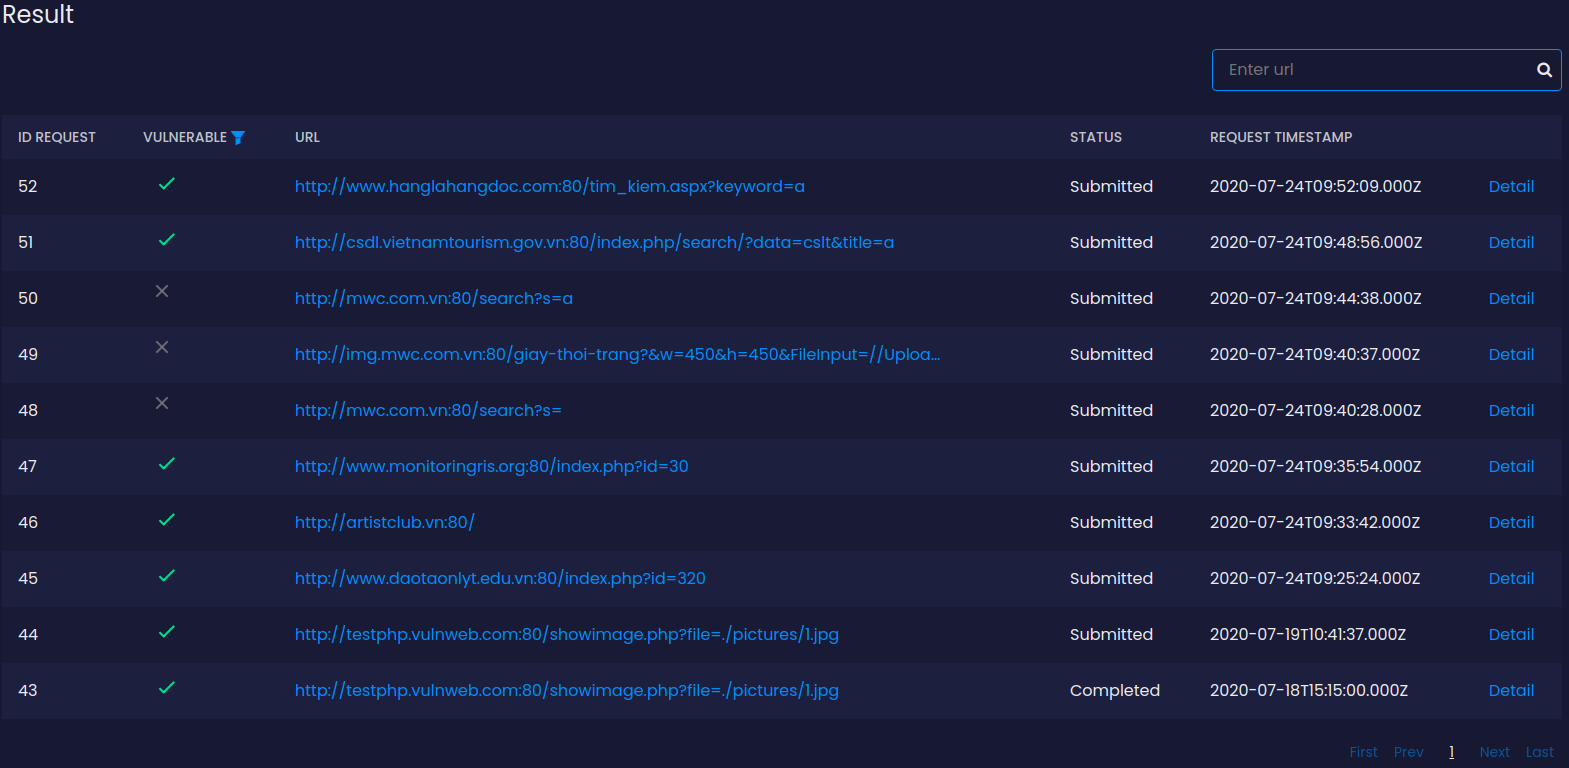
\includegraphics[scale=0.44,keepaspectratio=true]{images/result-ui.png}
    \caption{Giao diện trang kết quả kiểm thử ở UI ứng dụng webfuzzer}
    \label{fig:result-ui-ui}
\end{sidewaysfigure}
\FloatBarrier
Các thông tin cơ bản của một yêu cầu kiểm thử bao gồm ID, đường dẫn \acrshort{url}, thời điểm tạo, trạng thái và kết quả là có lỗ hổng hay không và các payload phát hiện được nếu có. Các thông tin này được truy vấn từ \acrshort{api} \colorbox{gray!30}{\texttt{GET /target}} theo ID của yêu cầu kiểm thử và hiển thị trên \acrshort{ui} như Hình \ref{fig:request-detail} sau.
\begin{figure}[H]
  \centering
    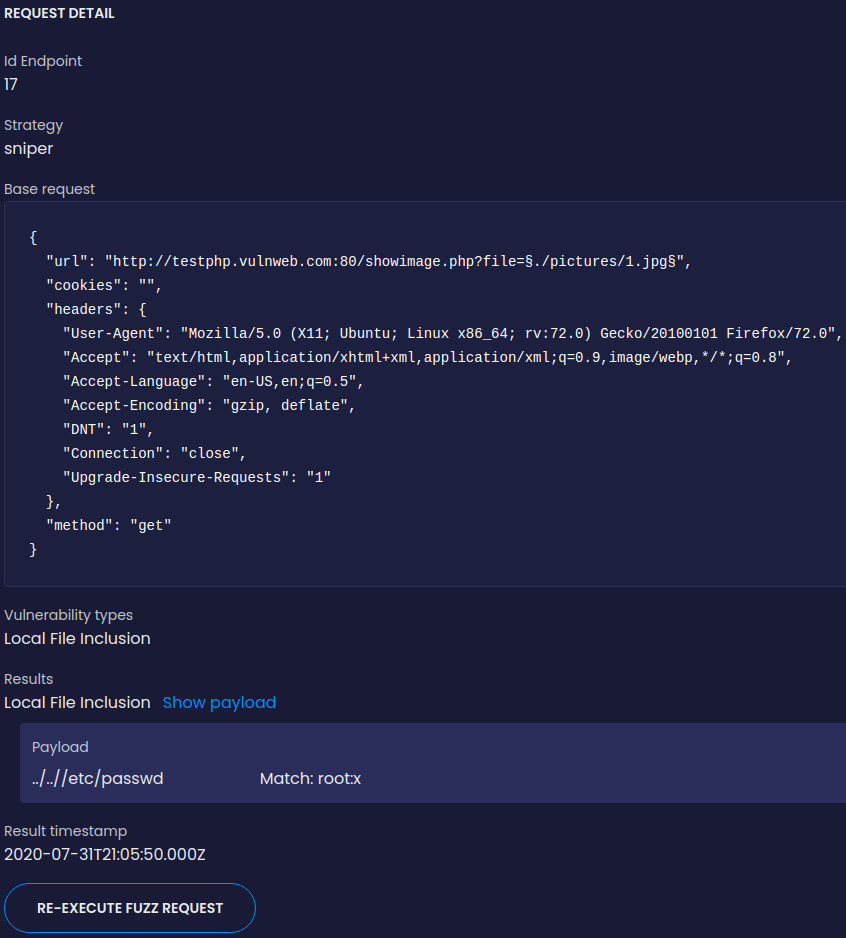
\includegraphics[width=1\textwidth,keepaspectratio=true]{images/request-detail.png}
  \caption{Thông tin chi tiết của một yêu cầu kiểm thử}
  \label{fig:request-detail}
\end{figure}
Chúng tôi hiện thực khung thông tin chi tiết của một yêu cầu kiểm thử trong component\\\texttt{RequestDetailComponent}. Mỗi thông tin hiển thị trong component này được đặt trong một thẻ \texttt{div} lần lượt từ trên xuống. Khung nội dung của request mẫu được chúng tôi tái sử dụng định dạng \acrshort{css} từ khung nội dung request mẫu ở trang bảng điều khiển. Khi người dùng nhấn nút ``\texttt{Show payload}'' bên cạnh loại lổ hổng ở khung kết quả kiểm thử, những payload phát hiện được lỗ hổng đó sẽ hiện ra. Chúng tôi chỉ lọc ra payload, những chuỗi so trùng và kết quả kiểm tra thời gian thực thi request kiểm thử (nếu có) trong kết quả kiểm thử tương ứng để hiển thị. Cuối cùng là nút (tái) thực thi một yêu cầu kiểm thử, nút này sẽ gọi đến \acrshort{api} \colorbox{gray!30}{\texttt{GET /fuzz}} thông qua hàm xử lí sự kiện \texttt{executeFuzzRequest} khi người dùng nhấn nút. Các thành phần trên của component \texttt{RequestDetailComponent} được hiện thực thông qua Đoạn mã \ref{lst:implement-RequestDetailComponent} sau.
\begin{lstlisting}[style=ES6, label={lst:implement-RequestDetailComponent}, caption={Hiện thực một số thành phần của component RequestDetailComponent}]
<div className="detail-item-title">Base request</div>
<div className="detail-item-content"><pre className="base-request">{JSON.stringify(JSON.parse(baseRequest), null, 2).replace(/\\\\xa7/gi, '§')}</pre></div>
...
<div className="result-content-item-title">Payload</div>
  {element.value ? element.value.map((item, idx) => (
    <div key={idx} className="result-content-item">
      <div className="result-content-item-content">{item.payload}
        <span style={{ marginLeft: '3rem' }} >
          {item.timebased ? 'Timebased: true' : null}
        </span>
        <span style={{ marginLeft: '3rem' }} >
          {item.matchList.length > 0 ? 'Match: ' + item.matchList.toString() : null}
        </span>
      </div>
    </div>
  )) : ''}
</div>
...
<div className="detail-item">
  <button disabled={this.checkDisableButton(requestId)} onClick={async () => this.executeFuzzRequest()}>{status == 'Completed' || status == 'Processing' ? 'Re-execute' : 'Execute'} fuzz request</button>
</div>
\end{lstlisting}
\subsection{Thanh điều hướng và các thành phần khác}
Thanh điều hướng của \acrshort{ui} được hiện thực bằng các component \texttt{Nav, Navbar, NavItem, NavLink} của thư viện reactstrap. Thuộc tính \texttt{vertical} của component \texttt{Nav} sẽ cố định thanh điều hướng dọc theo lề trái của trang web. Hai trang bảng điều khiển, kết quả kiểm thử được đưa vào thành hai thẻ trên thanh điều hướng dưới dạng các component \texttt{NavLink} như Đoạn mã \ref{lst:implement-nav-bar} sau. Kết quả hiện thực thanh điều hướng và thông báo đẩy được thể hiện trong Hình \ref{fig:notification-example}.
\begin{lstlisting}[style=ES6, label={lst:implement-nav-bar}, caption={Các thuộc tính props truyền vào component Nav}]
const navItems = [
  { to: '/', name: 'dashboard', exact: true, Icon: MdDashboard },
  { to: '/result', name: 'result', exact: false, Icon: MdWeb },
];
...
<Nav vertical>
  {navItems.map(({ to, name, exact, Icon }, index) => (
    <NavItem key={index} className={bem.e('nav-item')}>
      <NavLink
        id={`navItem-${name}-${index}`}
        className="text-uppercase"
        tag={NavLink}
        to={to}
        activeClassName="active"
        exact={exact}
      >
        <Icon className={bem.e('nav-item-icon')} />
        <span className="">{name}</span>
      </NavLink>
    </NavItem>
  ))}
</Nav>
\end{lstlisting}
\begin{figure}[H]
  \centering
    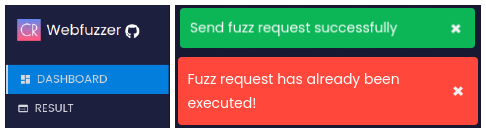
\includegraphics[width=0.9\textwidth,keepaspectratio=true]{images/notification-example.png}
  \caption{Thanh điều hướng và ví dụ thông báo đấy trên giao diện người dùng}
  \label{fig:notification-example}
\end{figure}
Các thông báo đẩy trên \acrshort{ui} của webfuzzer có hai kiểu, thành công (success) hoặc thất bại (error) như Hình \ref{fig:notification-example} trên. Định dạng của các kiểu này được thiết lập trong biến \texttt{NOTIFICATION\_SYSTEM\_STYLE} ở tập tin \texttt{src/utils/constants.js} trong thư mục gốc mã nguồn \acrshort{ui}. Chúng tôi sử dụng component \texttt{NotificationSystem} của thư viện\\\texttt{react-notification-system} để hiện thực các thông báo đẩy này. Các props chính mà component này nhận bao gồm nội dung thông báo (\texttt{message}), kiểu thông báo (\texttt{level}) và định dạng kiểu (\texttt{style}) như Đoạn mã \ref{lst:implement-notifications} sau.
\begin{lstlisting}[style=ES6, label={lst:implement-notifications}, caption={Các thuộc tính props truyền vào component NotificationSystem}]
this.notificationSystem.addNotification({
  message: 'Send fuzz request successfully',
  level: 'success',
  position: 'tc'
});
...
<NotificationSystem
  dismissible={false}
  ref={notificationSystem =>
    (this.notificationSystem = notificationSystem)
  }
  style={NOTIFICATION_SYSTEM_STYLE}
/>
\end{lstlisting}
Để phân trang các danh sách request mẫu và thông tin yêu cầu kiểm thử, chúng tôi sử dụng component \texttt{Pagination} có sẵn trong thư viện \texttt{react-js-pagination}. Component này nhận vào các props như danh sách phần tử cần hiển thị, tổng số lượng phần tử và số lượng phần tử ở mỗi trang, kèm theo các đoạn text hiển thị ở thao tác chuyển trang như trong Đoạn mã \ref{lst:implement-paging-component} sau.
\begin{lstlisting}[style=ES6, label={lst:implement-paging-component}, caption={Các thuộc tính props truyền vào component Pagination}]
<Pagination
  activePage={this.state.activePage}
  itemsCountPerPage={this.state.limit}
  totalItemsCount={this.state.totalRecord}
  pageRangeDisplayed={5}
  onChange={this.handlePageChange.bind(this)}
  prevPageText={'Prev'}
  nextPageText={'Next'}
  firstPageText={'First'}
  lastPageText={'Last'}
/>
\end{lstlisting}

\section{Cơ sở dữ liệu}
Dựa vào thiết kế đã đề ra ở \textbf{Chương 5}, chúng tôi hiện thực cấu trúc cơ sở dữ liệu của ứng dụng webfuzzer gồm ba bảng chính. Bảng \ref{tab:db-tables} dưới đây mô tả tên và chức năng của từng bảng trong lược đồ.
\begin{table}[ht]
    \centering
    \caption{Các bảng trong lược đồ quan hệ}
    \label{tab:db-tables}
    \begin{tabular}[ht]{lll}
        \toprule[1pt]\midrule[0.3pt]
            \textbf{Tên}& &\textbf{Mô tả}\\ 
        \midrule
            Endpoint& &Bảng Endpoint lưu lại các request mẫu mục tiêu được\\
            {}& &gửi đến máy chủ từ phần mở rộng Burp Suite\\
            \addlinespace
            Request& &Bảng Request lưu những yêu cầu kiểm thử một request mẫu \\
            {}& &trong bảng Endpoint của người dùng\\
            \addlinespace
            Result& &Bảng Result lưu kết quả kiểm thử chi tiết ứng với\\
            {}& &mỗi yêu cầu kiểm thử trong bảng Request\\
            \addlinespace
        \midrule[0.3pt]\bottomrule[1pt]
    \end{tabular}
\end{table}
\FloatBarrier
Hình \ref{fig:db-schema} dưới đây mô tả quan hệ giữa các bảng trong lược đồ.
\begin{figure}[H]
  \centering
    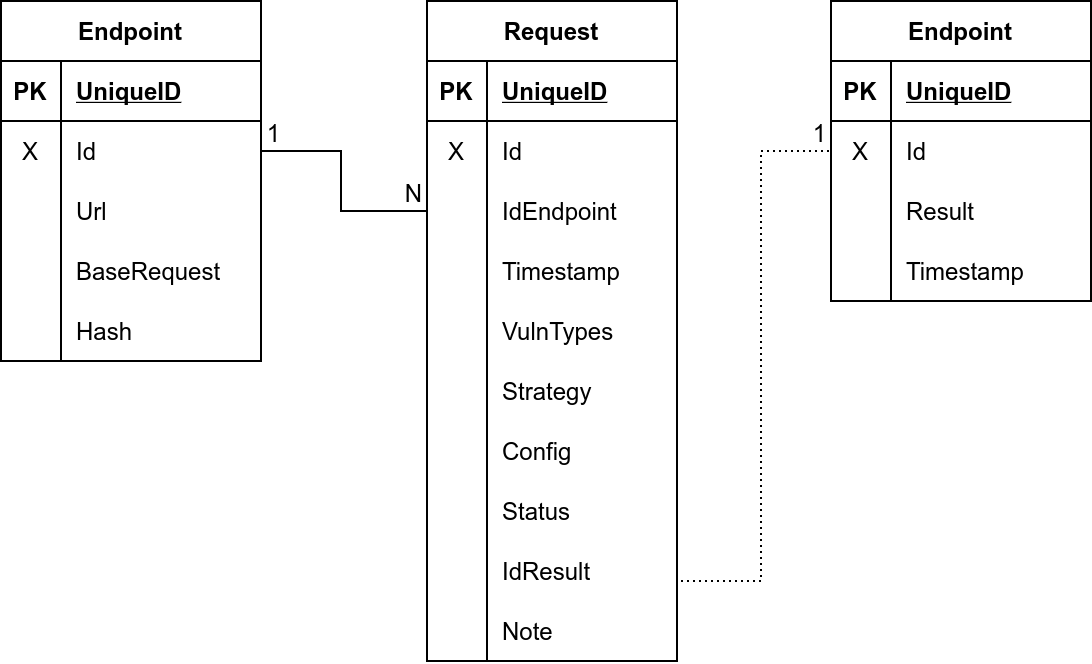
\includegraphics[width=0.75\textwidth,keepaspectratio=true]{images/database-design.png}
  \caption{Sơ đồ mối quan hệ giữa các bảng trong lược đồ}
  \label{fig:db-schema}
\end{figure}
Bảng \texttt{Endpoint} lưu trữ \acrshort{http} request mẫu được gửi từ phần mở rộng Burp Suite đến backend thông qua API \colorbox{gray!30}{\texttt{POST /}}. Request mẫu đó chứa dưới dạng chuỗi dữ liệu JSON trong trường \texttt{BaseRequest}. Trường \texttt{Url} chứa riêng \acrshort{url} của điểm cuối ứng dụng web mục tiêu để thuận lợi trong việc lọc ra những yêu cầu kiểm thử của cùng một trang web thông qua API \colorbox{gray!30}{\texttt{POST /target/search}}. Trường \texttt{Hash} chứa giá trị băm của chuỗi \texttt{BaseRequest}, đảm bảo không lưu hai request mẫu y hệt nhau gây dư thừa dữ liệu. Bảng \texttt{Request} chứa thông tin của các yêu cầu kiểm thử, trong đó trường \texttt{IdEndpoint} là khoá ngoại tham chiếu tới khoá chính \texttt{Id} của bảng \texttt{Endpoint} và trường \texttt{IdResult} là khoá ngoại tham chiếu tới khoá chính \texttt{Id} của bảng \texttt{Result} chứa kết quả kiểm thử (trong trường hợp có lỗ hổng). Mỗi bản ghi trong bảng \texttt{Request} chứa \acrshort{http} request mẫu gửi đến các điểm cuối của ứng dụng web mục tiêu, tập các lỗ hổng cần kiểm thử, trạng thái, và kết quả kiểm thử tương ứng, bao gồm danh sách lỗ hổng của điểm cuối đó và các payload phát hiện được. Trường \texttt{BaseRequest} của bảng \texttt{Endpoint}, trường \texttt{VulnTypes} của bảng \texttt{Request} và \texttt{Result} của bảng \texttt{Result} là các trường có kiểu chuỗi, chứa các giá trị kiểu đối tượng JSON đã được chuỗi hóa như đã đề cập trong phần thiết kế kiến trúc cơ sở dữ liệu ở trên.